\documentclass{article}
\usepackage{cmap}						% Улучшенный поиск русских слов в полученном pdf-файле
\usepackage[T2A]{fontenc}				% Поддержка русских букв
\usepackage{fontenc}				    % Поддержка русских букв
\usepackage{hyperref} 
\usepackage[utf8]{inputenc}				% Кодировка utf8
\usepackage[english, russian]{babel}	% Языки: русский, английский
\usepackage{amsthm,amsfonts,amsmath,amssymb,amscd} % Математические дополнения от AMS
\usepackage{graphicx} % Подключаем пакет работы с графикой

\usepackage{graphicx}  % Для вставки рисунков
\usepackage[update,prepend]{epstopdf} % EPS-рисунки конвертируются в PDF
\usepackage{wrapfig} % Обтекание рисунков текстом
\usepackage[usenames,dvipsnames,svgnames,table,rgb]{xcolor}
\usepackage{float}

 \usepackage{geometry} % Простой способ задавать поля
 \geometry{top=30mm}
 \geometry{bottom=25mm}
 \geometry{left=20mm}
 \geometry{right=15mm}

\newcolumntype{C}[1]{>{\centering\arraybackslash}m{#1}}
 

\begin{document}

\begin{titlepage}  

\begin{center}  

\large Национальный исследовательский университет \\"Высшая школа экономики"\\[0.5cm]

\large Факультет компьютерных наук\\

\large Департамент анализа данных и искусственного интеллекта\\[4cm]

\huge Домашнее задание №1\\
\large по анализу и разработке данных\\[4cm]

\end{center}

\begin{flushleft}
\large Выполнили студенты БПМИ133:\\
\large \bf{Стеценко Макар}\\
\large \bf{Корытова Александра}\\
\large \bf{Милеев Алексей}\\[5cm]
\end{flushleft}

\begin{center}
\large Москва 2015
\end{center}

\end{titlepage}

\newpage

1. В настоящих данных приводится статистика по NEA (Near Earth Objects) и кометам, обнаруженным иследовательской миссией NEOWISE под руководством NASA. Near-Earth Objects - это кометы и астероиды, которые были притянуты гравитационным полем ближайщих планет, в следствии чего они смогли сблизиться с Землей. \\[0.3cm]



Каждый объект описывается следующим набором признаков:

\begin{itemize}
\item {Discovery Date [Дата открытия]} 

Качественный признак в формате YYYY-MM-DD

\item {H (mag) [Магнитуда]}

Количественный признак, абсолютная величина

С помощью абсолютной магнитуды вычисляется диаметр астероида, чем ниже значение H, тем больше размер объекта.

\item {MOID (AU) - Minimum Orbit Distance [Минимальная дистанция орбиты]}

Количественный признак, измеряемый относительно AU (The astronomical unit).

//AU - астрономическая единица измерения длины, приближенно показывающая расстояние между Землей и Солнцем. Равна 149597870700 метров (примерно 150 млн км).

Minimum orbit intersection distance (MOID) - мера, используемая в астрономии для оценки потенциальных сближений и рисков столкновений между астрономическими объектами.

\item {q (AU) perihelion distance}

Количественный признак

Perihelion - точка на орбите планеты, кометы или другого объекта, расстояние от которой до Солнца минимально.

\item {Q (AU) aphelion distance}

Количественный признак

Aphelion - точка, в которой небесное тело максимально удалено от Солнца.

\item {period (yr) [Период]}

Количественный признак, показывающий период обращения объекта вокруг Солнца, измеряется в годах.


\item {PHA (Potentially Hazardous Asteroids)}

Признак, показывающий принадлежит ли астероид к классу PHA. 
Принимает два значения (Y/N), для удобства можно считать количественным. 

\item {Orbit Class [Класс орбиты]}

Качественный признак, множество принимаемых значений: \{Apollo, Aten, Amor, Atiras\}.\\[0.3cm]

\end{itemize} 

2. Предметная область\\[0.15cm]

Научный интерес к таким объектам проявлен во многом из-за их происхождения. Так, например, астероиды по сути являются уцелевшими осколками после формирования нашей солнечной системы. Поскольку эти объекты могут столкнуться, они оказывали и будут оказывать влияние на биосферу Земли. Так же астероиды являются богатым источником ресурсов. Выяснилось, что минеральных запасов в астероидном поисе Марса и Юпитера хватит, чтобы каждому человеку на Земле дать 100 миллиардов долларов.

По имеющимся данным можно пробовать строить модели для определения принадлежности небесного объекта к классу PHA. \\[1cm]

Источник: \href{http://neo.jpl.nasa.gov/stats/wise/}{http://neo.jpl.nasa.gov/stats/wise/}. 

\vspace{.2cm}
\large \textbf{Домашнее задание №2}
\vspace{.2cm}

1. Был выбран количественный признак H (mag) [Магнитуда]. Поскольку этот признак позволяет определить размер исследуемого объекта, то его подробное изучение позволит лучше понять, каких размеров достигают наиболее встречаемые астероиды. Построим гистрограму: 

\begin{figure}[H] 
\centering
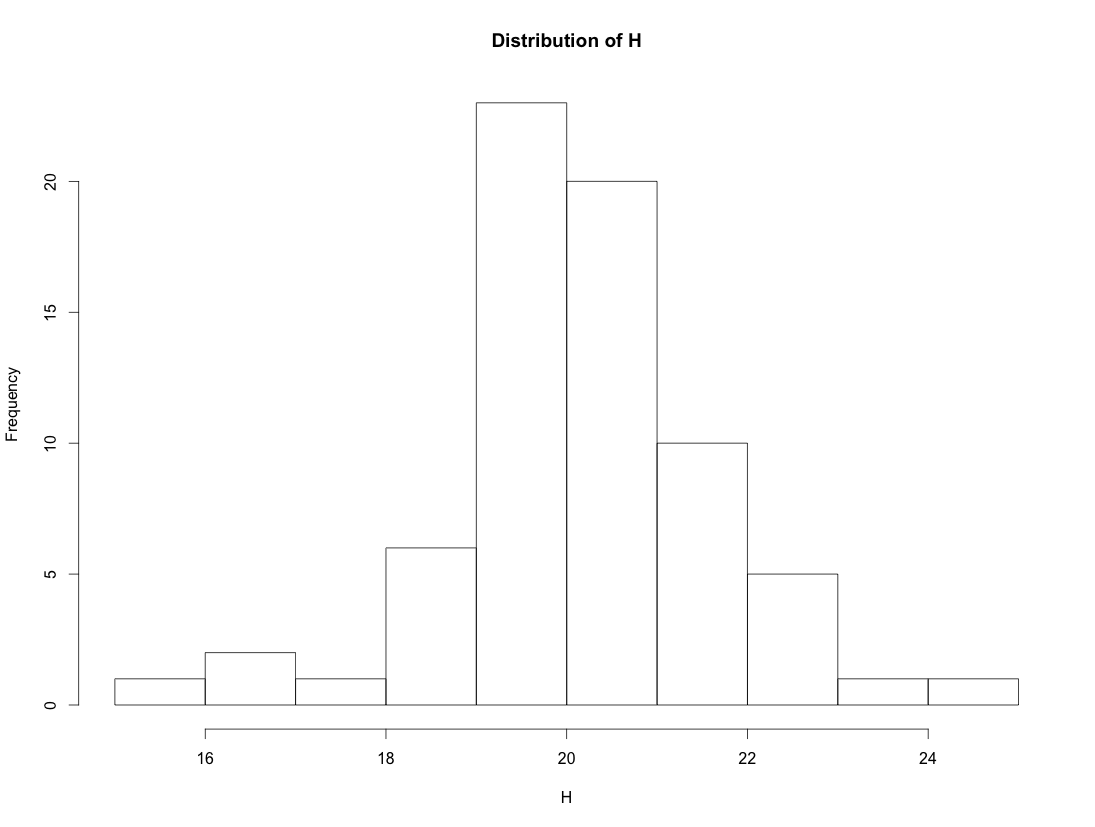
\includegraphics[scale=0.4]{2_hist.png}
\caption{Гистограма для признака H (mag)}
\label{fig :metka1}
\end{figure}

Полученная гистограмма позволяет нам предположить, что распределение признака H похоже на нормальное. Так же, понять, в каком диапазоне лежат наиболее встречаемые значения H, примерно от 19 до 21, этот факт подтвердится, когда мы найдем моду. Построим бокс-плот:

\begin{figure}[H] 
\centering
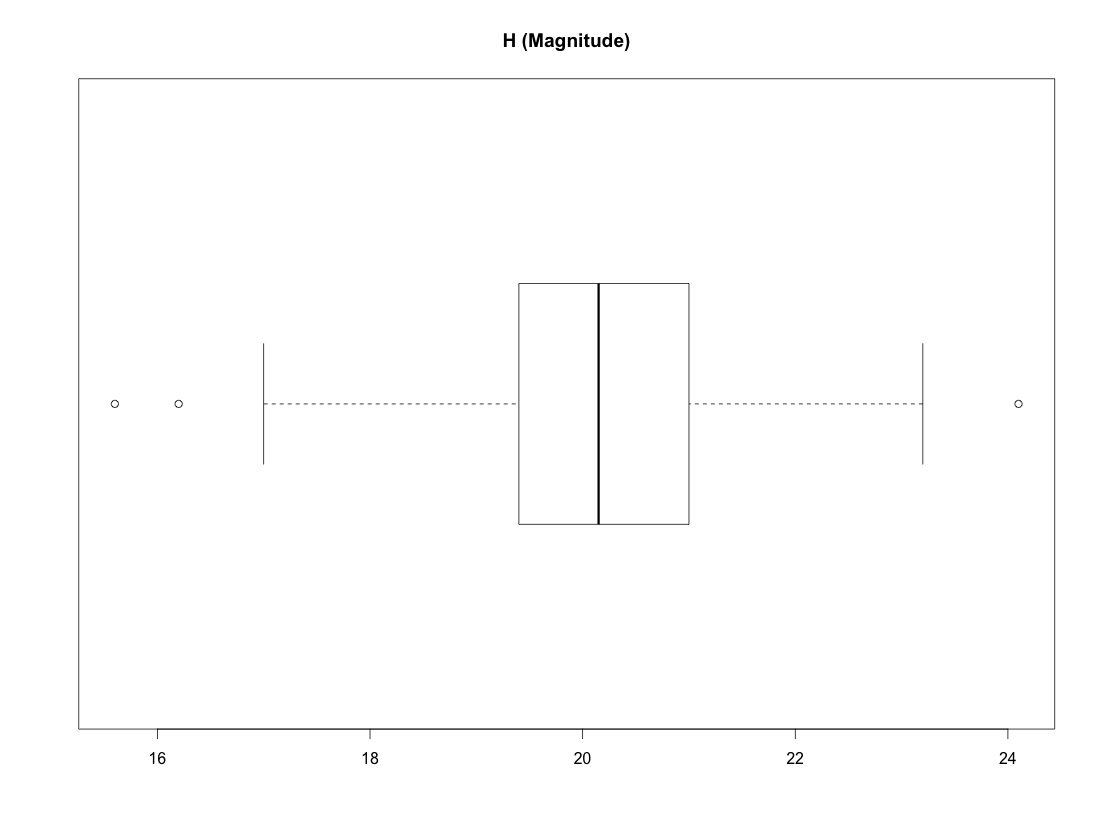
\includegraphics[scale=0.4]{2_box.png}
\caption{Бокс-плот для H (mag)}
\label{fig :metka1}
\end{figure}

Видно, что у нас есть 3 выброса, которые отмечены белыми кружками. Так же видно значение медианы.

Найдем среднее значение, моду и медиану

\begin{center}
  \begin{tabular}{| C{2.5cm} | C{2.5cm} | C{2.5cm} | @{}m{0pt}@{}}
    \hline
    Среднее & Медиана & Мода &\\[0.5em] \hline
    20.21 & 20.15 & 19.7 и 20.7 &\\[0.5em]   
    \hline
  \end{tabular}
\end{center}

Как видно, найденные значения не равны, это свидетельствует о том, что величина H не подчиняется нормальному распределению, а немного отклоняется от него.


\end{document}
